\documentclass[11pt]{article}
\usepackage[a4paper,width=150mm,top=25mm,bottom=25mm]{geometry}
\usepackage[spanish]{babel}
\usepackage[utf8]{inputenc}
\usepackage{fancyhdr}
\usepackage{xhfill}
\usepackage{nameref}
\pagestyle{fancy}

\usepackage{graphicx}
\usepackage{tabularx}
\usepackage{listingsutf8}
\usepackage{color}
\usepackage{import}
\usepackage{amsmath}
\usepackage{enumitem}

\definecolor{mygreen}{rgb}{0,0.6,0}
\definecolor{mygray}{rgb}{0.5,0.5,0.5}
\definecolor{mymauve}{rgb}{0.58,0,0.82}
\renewcommand{\lstlistingname}{Listado}
\lstset{
  backgroundcolor=\color{white},   % choose the background color; you must add \usepackage{color} or \usepackage{xcolor}; should come as last argument
  basicstyle=\footnotesize,        % the size of the fonts that are used for the code
  breakatwhitespace=false,         % sets if automatic breaks should only happen at whitespace
  breaklines=true,                 % sets automatic line breaking
  captionpos=b,                    % sets the caption-position to bottom
  commentstyle=\color{mygreen},    % comment style
  deletekeywords={...},            % if you want to delete keywords from the given language
  escapeinside={\%*}{*)},          % if you want to add LaTeX within your code
  firstnumber=1,                   % start line enumeration with line 1
  frame=single,	                   % adds a frame around the code
  inputpath=./../,
  inputencoding=utf8/latin1,
  keepspaces=true,                 % keeps spaces in text, useful for keeping indentation of code (possibly needs columns=flexible)
  keywordstyle=\color{blue},       % keyword style
  language=Java,                 % the language of the code
  morekeywords={*,...},            % if you want to add more keywords to the set
  numbers=left,                    % where to put the line-numbers; possible values are (none, left, right)
  numbersep=5pt,                   % how far the line-numbers are from the code
  numberstyle=\tiny\color{mygray}, % the style that is used for the line-numbers
  rulecolor=\color{black},         % if not set, the frame-color may be changed on line-breaks within not-black text (e.g. comments (green here))
  showspaces=false,                % show spaces everywhere adding particular underscores; it overrides 'showstringspaces'
  showstringspaces=false,          % underline spaces within strings only
  showtabs=false,                  % show tabs within strings adding particular underscores
  stepnumber=2,                    % the step between two line-numbers. If it's 1, each line will be numbered
  stringstyle=\color{mymauve},     % string literal style
  tabsize=2,	                   % sets default tabsize to 2 spaces
  title=\lstname,                   % show the filename of files included with \lstinputlisting; also try caption instead of title
  xleftmargin=15pt,
  xrightmargin=15pt
}

\fancyhead{}
\fancyhead[R]{Obligatorio}
\fancyhead[L]{Teoría de la Computación}



\graphicspath{{img/}}

\newcommand{\BigO}[1]{\ensuremath{\mathrm{O}\bigl(#1\bigr)}}
\newcommand{\BigT}[1]{\ensuremath{\mathrm{\Theta}\bigl(#1\bigr)}}
\newcommand{\type}[1]{\mbox{\textbf{#1}}}
\newcommand{\call}[1]{\mbox{\texttt{#1}}}

\overfullrule=2cm

\begin{document}

\begin{titlepage}
    \begin{center}
        
\includegraphics[width=0.7\textwidth]{ucu}

	\vspace*{5cm}

        \Huge
        \textbf{Obligatorio}

        \vspace{0.5cm}
        \LARGE
	Teoría de la Computación

        \vspace{3.5cm}

        Lois, Lucas

        Maresca, Santiago

        Silveira, Marco

        \vfill

        \Large
        Universidad Católica del Uruguay\\
        22 de Noviembre, 2019

    \end{center}
\end{titlepage}



\section{Armado de un Árbol-KDR}
\begin{lstlisting}[language=Python]
	
def makeKDRTree(points, r, dim = 0):
	if not points:
		return None # Empty trees are None
	elif len(points) == 1:
		return tuple(points) # Leaf nodes have one point.

	# Obtenemos las r medianas, para las dimensiones dim, dim+1, ..., dim+(r-1)
	medians = getMedians(points, r, dim)

	partitions = [None] * (2**r + 1) # Tendremos 2**r particiones (hijos)
	partitions[0] = medians
	i = 1
	for criteria in it.product([False, True], repeat = r):  # 2^r iteraciones
		partition = [p for p in points if matches_criteria(criteria, medians, p, dim)] # n iteraciones
		partitions[i] = makeKDRTree(partition, r, (dim+r) % len(points))
		i += 1

	return tuple(partitions)
	\end{lstlisting}
\textbf{ Orden de tiempo de ejecución del algoritmo : }
{Mejor de los casos: points es nulo o es una tupla de largo uno : 
el algoritmo tendrá orden de ejecución : O(1).
Caso promedio : 



}

	\section{Búsqueda de un Árbol-KDR}
	\begin{lstlisting}[language=Python]
	def searchKDRTree(kdrTree, r, point, dim = 0):
		if (kdrTree is None):
			return False
		elif len(kdrTree) == 1:
			return kdrTree[0] == point
		medians = kdrTree[0]
		i = 1
		for criteria in it.product([False, True], repeat = r):  # 2^r iteraciones
			if (matches_criteria(criteria, medians, point, dim)):
				# go to this subtree
				chosen_subtree = kdrTree[i]
				return searchKDRTree(chosen_subtree, r, point, dim+r)
			i += 1
	
		return False
		\end{lstlisting}
	\textbf{ Orden de tiempo de ejecución del algoritmo : }
		{Mejor de los casos: points es nulo o es una tupla de largo uno : 
		el algoritmo tendrá orden de ejecución : O(1).
		Caso promedio : 
		
		
		
		}


% \begin{algorithm}
% \caption{Busca una tupla de largo R en un arbol KDR}
% \label{alg:busqueda-kdr}
% \begin{algorithmic}[1]
% 	\Require El árbol kdr debe estar creado
% \Procedure{searchKDRTree}{kdrTree, r, point, dim = 0}
% \If {kdTree == nulo}
% \State {devolver Falso}
% \Else{}
% \If {kdTree == nulo}
% \State devolver kdrTree[0] == point

% medians =kdrTree[0]
% \ForAll{(criteria,) $\in$ productoCartesiano(false,true,r)}
% 	\State s.put(``\{i\}) \{evento.getNombre()\} \{evento.getCuando()\}'');
% \EndFor
% \EndProcedure
% \end{algorithmic}
% \end{algorithm}

% El algoritmo \ref{alg:crear-kdr} muestra la respuesta del sistema cuando se detalla un id de evento.
% En este caso se representa, para el evento determinado, qué entras están disponibles (mediante id),
%     así como su precio.

\section{Análisis Experimental}

\begin{figure}
  \begin{center}
  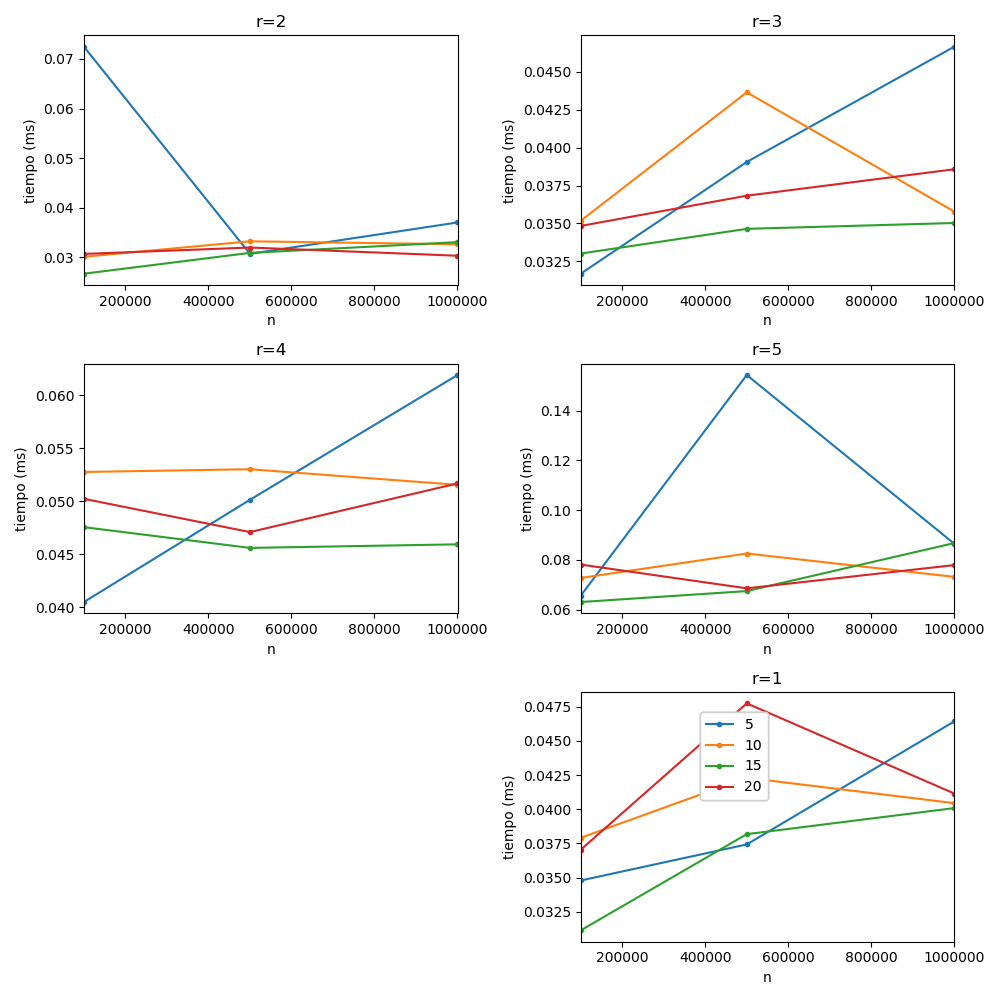
\includegraphics[width=\textwidth]{buscar_pos_n}
  \caption{Tiempo de búsqueda (positiva)
    según n, para distintos valores de r y k.}
  \label{fig:buscar-pos}
  \end{center}
\end{figure}


\begin{figure}
  \begin{center}
  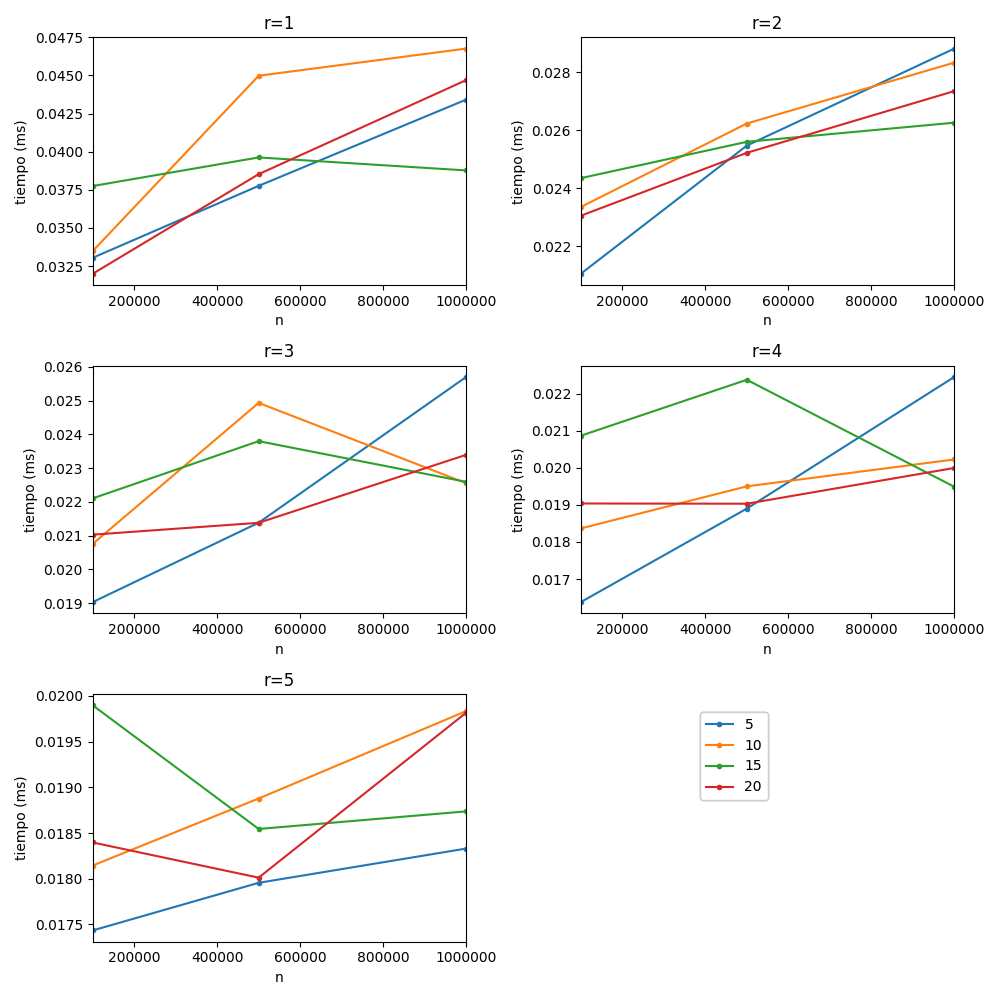
\includegraphics[width=\textwidth]{buscar_neg_n}
  \caption{Tiempo de búsqueda (negativa)
    según n, para distintos valores de r y k.}
  \label{fig:buscar-neg}
  \end{center}
\end{figure}

En las figuras \ref{fig:buscar-pos} y \ref{fig:buscar-neg} podemos
ver un crecimiento ligeramente cercano al logarítmico (que con tan solo 3
valores\footnote{Como se indica en la consigna} para \(n\) es difícil
distinguir).

La diferencia para distintos r (dado un k) se observa en la figura
\ref{fig:buscar}, y en todos los casos podemos observar que el árbol
con mayor r tiene un mejor rendimiento para las búsquedas tanto positivas como
negativas.

\begin{figure}
  \begin{center}
  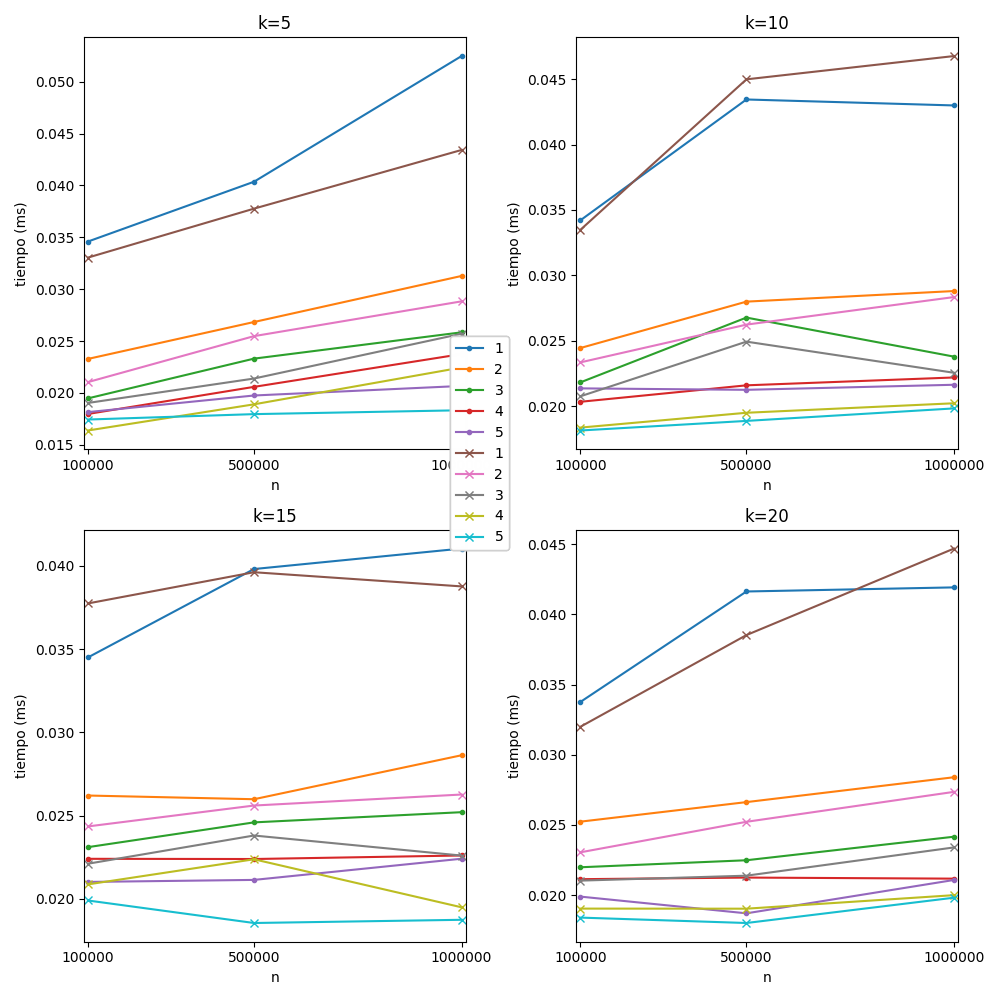
\includegraphics[width=\textwidth]{buscar_n}
  \caption{Tiempo de búsqueda (positiva y negativa)
    según n, para distintos valores de r y k.}
  \label{fig:buscar}
  \end{center}
\end{figure}

Esto se alinea con el desarrollo teórico, ya que \(r\) indica el factor de
ramificación, y cuanto mayor sea menos niveles debe recorrer hasta completar la
búsqueda.

Se observa una pequeña superioridad de las búsquedas negativas ante las positivas,
pero la diferencia no es significativa.

\begin{figure}
  \begin{center}
  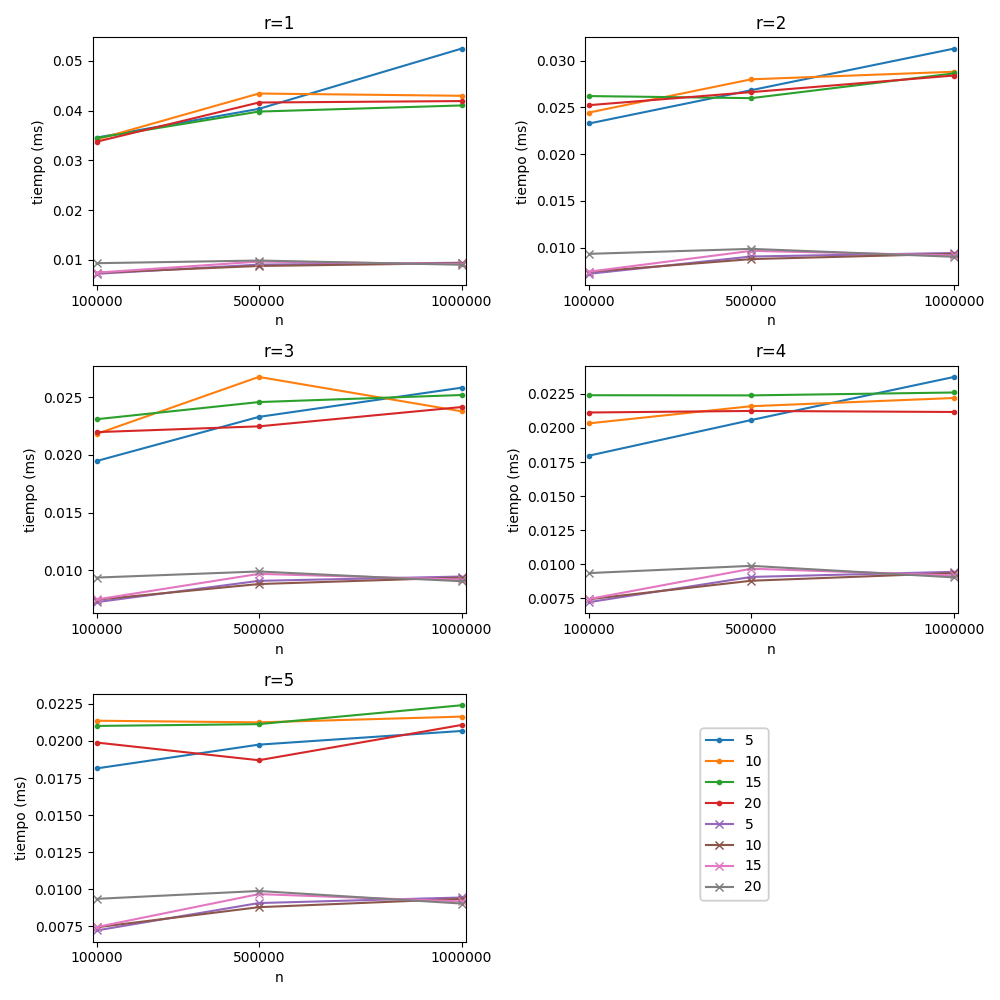
\includegraphics[width=\textwidth]{buscar_pos_kd_n}
  \caption{Tiempo de búsqueda (positiva)
    según n, para distintos valores de r y k, comparado con el árbol kd.}
  \label{fig:pos-kd}
  \end{center}
\end{figure}


\begin{figure}
  \begin{center}
  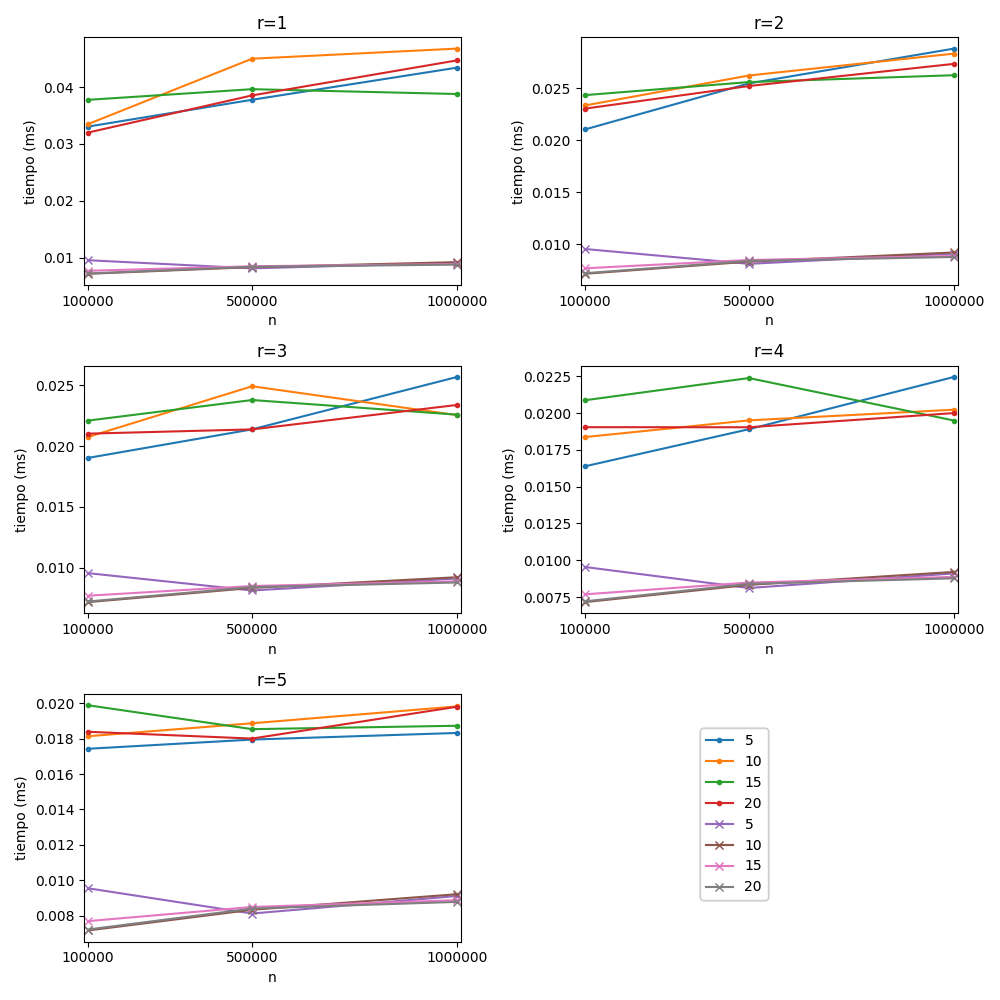
\includegraphics[width=\textwidth]{buscar_neg_kd_n}
  \caption{Tiempo de búsqueda (negativa)
    según n, para distintos valores de r y k, comparado con el árbol kd.}
  \label{fig:neg-kd}
  \end{center}
\end{figure}


En las figuras \ref{fig:pos-kd} y \ref{fig:neg-kd} podemos observar
una clara superioridad del árbol kd de búsqueda, logrando sus
búsquedas siempre por debajo de los 0.010ms, y esto se mantiene para
todo k y todo r. Ente los árboles kdr se observa variabilidad pero no
es significativa. Aún más, la creación de árboles
(fig. \ref{fig:armado}) muestra que la creación de arboles kd es
también superior, lo que es de esperar por la mayor complejidad del
algoritmos al tener que comparar r medianas.


\begin{figure}
  \begin{center}
  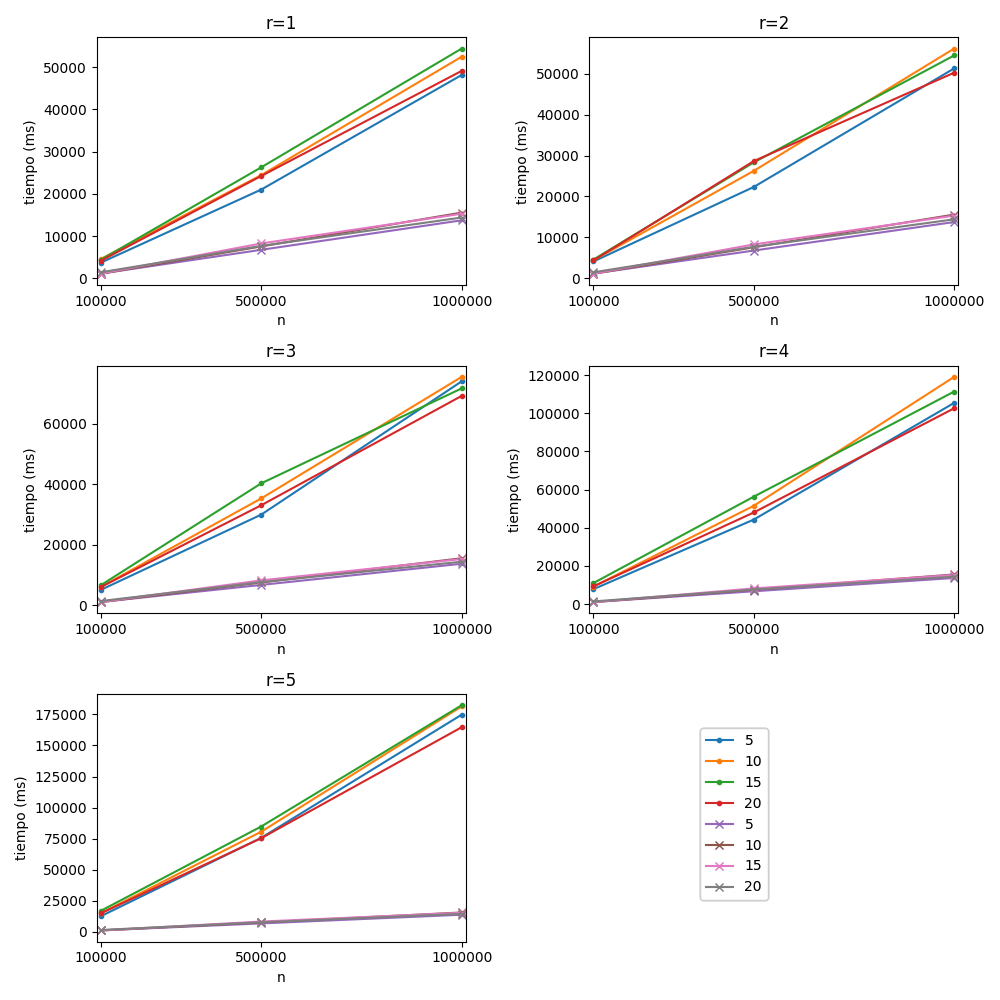
\includegraphics[width=\textwidth]{armado_n}
  \caption{Tiempo de creación de los arboles kd y kdr
    según n, para distintos valores de r y k.}
  \label{fig:armado}
  \end{center}
\end{figure}

\section{Conclusiones}
La hipótesis del proyecto plantea si resulta más eficiente la
búsqueda al particionar el subconjunto de puntos en más de una
dimensión.
Fue necesario analizar empíricamente ambos algoritmos, para poder
concluir qué sucede eventualmente.
Podemos apreciar, luego del análisis, que la búsqueda KDR,
mas allá de su aparente ventaja por reducir el número de niveles en la
búsqueda (particionando al conjunto en \(2^r\) subconjuntos), no logra
mejorar los tiempos que da el árbol kd tradicional,
y su construcción es además aún peor que el kd.

De todas formas, creemos que el proyecto fue muy productivo para poner
en práctica los conceptos aprendidos en clase, desde escribir el
código del algoritmo,  
analizar el orden de tiempo de ejecución, hasta ejecutar pruebas y
simulaciones.
Algunas obstáculos que se nos presentaron fueron la función
matches\_criteria, que inicialmente presentaba orden exponencial, lo
cual aumentaba el orden de tiempo de ejecución y hacía aún mayor la
brecha entre ambos,
como también, realizar las simulaciones, que resultaron llevar más
tiempo de lo dimensionado.

Asimismo, creemos haber realizado un buen análisis para comprender y
afirmar que la performance del algoritmo de búsqueda KD presenta
en todos los casos estudiados una mejor solución a la búsqueda multidemensional.


\end{document}
